
\chapter{Evaluación\label{chap:Evaluaci=0000F3n}}

En este capitulo se presenta la evaluación del enfoque propuesto con
el objetivo de analizar el desempeño de las técnicas de aprendizaje
de máquina utilizadas para predecir propiedades no-funcionales en
dispositivos móviles. Con este fin, se crearon tres casos de estudio
sobre los que se construyen y evalúan modelos de predicción.

El capítulo se organiza de la siguiente manera: en la sección \ref{sec:Metodolog=0000EDa-de-Evaluaci=0000F3n}
se detalla el proceso de evaluación propuesto. En las secciones \ref{subsec:Escenario-4:-Multiplicaci=0000F3n},~\ref{subsec:Escenario-1:-Algoritmos}~y~\ref{subsec:Escenario-2:-Servicios}
se presentan los escenarios de estudio considerados, brindando una
descripción de los componentes involucrados, las mediciones obtenidas
y los modelos de predicción construidos y evaluados. Los resultados
y discusión son expuestos en la sección \ref{sec:Analisis-y-discusi=0000F3n}
para analizar el desempeño de las técnicas de regresión sobre cada
caso de estudio. Finalmente en la sección \ref{sec:Conclusiones}
se presentan las conclusiones del capítulo. 


\section{Proceso de Evaluación\label{sec:Metodolog=0000EDa-de-Evaluaci=0000F3n}}

El proceso de evaluación, ilustrado en la Figura~\ref{fig:Proceso-de-evaluaci=0000F3n},
consiste en aplicar el enfoque sobre diferentes propiedades y grupos
de componentes, y evaluar los modelos de predicción con diferentes
métricas para analizar el desempeño de las distintas técnicas de aprendizaje
incluidas en la herramienta.

\begin{figure}
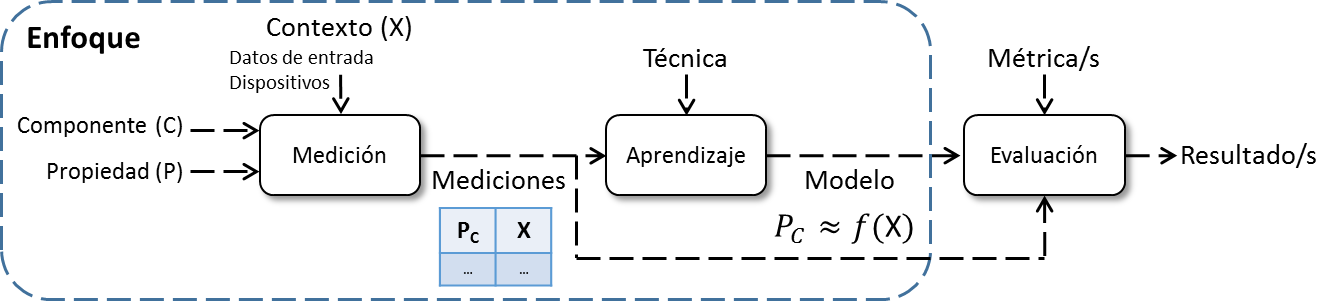
\includegraphics[scale=0.6]{images/Proceso-de-evaluacion}

\caption{Proceso de evaluación\label{fig:Proceso-de-evaluaci=0000F3n}}
\end{figure}


La calidad de los modelos será evaluada a través de dos métricas
que computan de forma distinta el error de predicción. Cada modelo
$f$ es construido por una técnica \emph{$T$} (regresión lineal,
red neuronal, etc.) que se aplica sobre un dataset de mediciones para
predecir una propiedad $P$ (tiempo de respuesta, precisión) de un
componente $C$. El proceso de evaluación consiste en tomar el conjunto
de mediciones usado para el aprendizaje de modelos de predicción y
utilizarlos para validar estos modelos a través las métricas de evaluación. 

Para un análisis más profundo sobre las distintas técnicas y su desempeño,
se usaron tres escenarios o casos de estudio de distintos dominios:
algoritmos para multiplicación de matrices, algoritmos para el problema
del viajante, y componentes para detección de rostros en imágenes.
Cada escenario comprende un conjunto de componentes y datos de entrada
a partir de lo cual se obtiene un dataset de mediciones. En todos
los escenarios se considera el tiempo de respuesta como propiedad
a medir y predecir. En el segundo y tercer caso de estudio, se considera
adicionalmente como propiedad la optimalidad o precisión en el resultado
arrojado por el componente.

El cuadro \ref{tab:Especificaciones-de-los-1} presenta la lista de
dispositivos sobre los que se han realizado las pruebas, con sus características
mas relevantes.

\begin{table}[H]
\begin{doublespace}
\begin{centering}
\resizebox{1\textwidth}{!}{%
\begin{tabular*}{20cm}{@{\extracolsep{\fill}}|c|c|c|c|c|}
\hline 
{\large{}Dispositivo} & {\large{}Frecuencia de CPU} & {\large{}Nucleos de CPU} & {\large{}Memoria RAM} & {\large{}Sistema Operativo}\tabularnewline
\hline 
{\large{}Lenovo K3 Note} & {\large{}1.7Ghz} & {\large{}Octa-Core} & {\large{}2GB} & {\large{}Android 5.0}\tabularnewline
\hline 
{\large{}Samsung Galaxy S3} & {\large{}1.4 Ghz, } & {\large{}Quad-Core} & {\large{}1GB} & {\large{}Android 4.3}\tabularnewline
\hline 
{\large{}Samsung Galaxy S4} & {\large{}1.9Ghz} & {\large{}Quad-Core} & {\large{}2GB} & {\large{}Android 4.2.2}\tabularnewline
\hline 
{\large{}Samsung Galaxy S5} & {\large{}2.5Ghz} & {\large{}Quad-Core} & {\large{}2GB} & {\large{}Android 4.4.2}\tabularnewline
\hline 
{\large{}Samsung Galaxy S6} & {\large{}2.1Ghz} & {\large{}Octa-Core} & {\large{}3GB} & {\large{}Android 5.0}\tabularnewline
\hline 
\end{tabular*}}
\par\end{centering}
\end{doublespace}

\caption{Características de los dispositivos móviles utilizados.\label{tab:Especificaciones-de-los-1}}
\end{table}



\subsection{Métricas de evaluación\label{subsec:M=0000E9tricas-de-evaluaci=0000F3n}}

Existe una gran cantidad de métricas por las cuales pueden evaluarse
y compararse los modelos de regresión. Todos los indicadores comparan
los valores reales con sus estimaciones, pero lo hacen de una manera
ligeramente diferente. 

\emph{\ac{MAE}} es el promedio del error absoluto (diferencia entre
los valores predichos y los observados), e indica cuán grande es el
error que puede esperarse de la predicción. Al tratarse de una métrica
basada en el error medio puede subestimar el impacto de errores grandes
pero infrecuentes. Si el análisis se centra demasiado en la media
arrojará conclusiones precipitadas, por lo tanto para ajustar errores
grandes y raros, se calcula el error cuadrático medio (\ac{RMSE}).
La ecuación de la métrica \ac{RMSE} es:

\[ \sqrt{\frac{1}{N}\sum_{i=1}^{N}{f_i-y_i}^2}
\]

La misma nos permite llegar a una medida del tamaño del error que
da más peso a los errores grandes e infrecuentes que la media. 

El coeficiente de correlación de Pearson es una medida de la relación
lineal entre dos variables aleatorias cuantitativas, independientemente
de la escala de medida de las mismas. El coeficiente de correlación
(\ac{CC}) es analizado en conjunto con el indicador \emph{\ac{RMSE}}
ya que existe una estrecha relación entre ambos. Por ejemplo, si \emph{\ac{CC}}
es 1, \emph{\ac{RMSE}} debe ser 0, ya que todos los puntos se encuentran
en la línea de la función de regresión; cuanto más cercano sea el
valor de \emph{\ac{CC}} a 1 o -1, más próximos son los valores observados
a la línea de predicción, y por tanto menor será el error absoluto
reflejado en \emph{\ac{RMSE}}. La fórmula de CC entre dos variables
\emph{x} e \emph{y} se define como:

\[
\frac{n\sum x_{i}y_{i}-\sum x_{i}\sum y_{i}}{\sqrt{n\sum x_{i}^{2}-(\sum x_{i})^{2}}\sqrt{n\sum y_{i}^{2}-(\sum y_{i})^{2}}}
\]



\subsection{Parámetros de configuración de las técnicas\label{subsec:Par=0000E1metros-de-configuraci=0000F3nde}}

La obtención de un modelo de calidad tiene lugar a partir de la optimización
de los parámetros de configuración de la técnica de regresión. Estos
parámetros pueden tomar distintos valores adaptándose a condiciones
particulares de los datos, generando modelos mas precisos que otros.
El Cuadro \ref{tab:Par=0000E1metros-de-configuraci=0000F3n} presenta
la lista completa de parámetros de configuración de cada técnica,
el valor por defecto adoptado para cada una y el rango de valores
con el cual se busca el modelo de mayor precisión. 

\begin{table}[H]
\begin{centering}
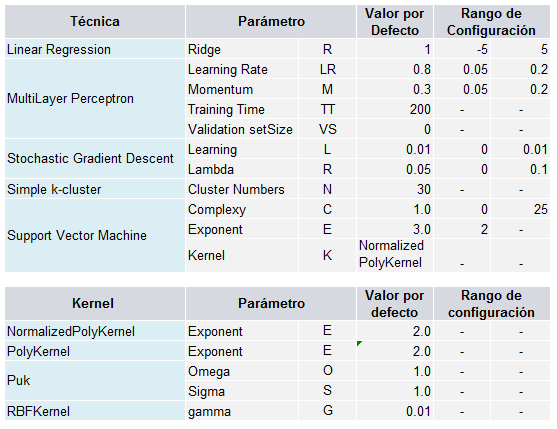
\includegraphics[scale=0.5]{images/configuration-parameters}
\par\end{centering}

\caption{Parámetros de configuración de las técnicas de regresión \label{tab:Par=0000E1metros-de-configuraci=0000F3n}}
\end{table}


El proceso de optimización de las técnicas utiliza el rango de configuración
establecido para iterar en pasos tomando valores intermedios y evaluando
la calidad del modelo generado con tales configuraciones. Los resultados
se comparan entre sí para determinar la mejor configuración para un
dataset y propiedad a predecir particular. 

Los rangos para cada técnica se establecieron tras un análisis de
la influencia de estos valores sobre los datos. Los rangos de prueba
se definieron de manera aleatoria, al mismo tiempo que el análisis
de un rango ya propuesto servía como base para definir uno nuevo.
Por otro lado, los valores elegidos por defecto fueron tomados de
los valores propuestos por la herramienta Weka, a excepción del parámetro
\emph{Training Time} de la técnica \emph{MultiLayer Perceptron} que
fue reducido de 500 a 200 para mejorar el tiempo de ejecución del
algoritmo. 

En las siguientes secciones se presenta la aplicación del enfoque
sobre distintos escenarios. Por cada escenario se describen los componentes
involucrados, el proceso de medición de los mismos, los datos obtenidos
con los que se entrenan las técnicas de predicción, y los resultados
de la evaluación de los modelos obtenidos.


\section{Caso de estudio 1: algoritmos para multiplicación de matrices\label{subsec:Escenario-4:-Multiplicaci=0000F3n}}

La multiplicación o producto de matrices es una operación matemática
entre dos matrices $A:=(a_{i,j})_{m\times n}$ y $B:=(b_{i,j})_{n\times p}$
con la que se obtiene una nueva matriz $C:=(c_{i,j})_{m\times p}$,
donde cada número real $c_{i,j}$ de $C$ esta definido por: $c_{i,j}=\stackrel[r=1]{n}{\sum}a_{i,r}b_{r,j}$.
El producto de matrices es un problemas de clase P, que a diferencia
de los problemas NP tienen complejidad temporal polinómica. El producto
entre matrices no es conmutativo, depende del orden de las matrices
involucradas, y sólo es posible si el número de filas de la primera
matriz es igual al número de columnas de la segunda. 

Un dataset sobre este dominio ha sido formado tras la ejecución y
medición del tiempo de ejecución de diferentes algoritmos de multiplicación
de matrices, con tamaños variados de matrices. Los componentes (algoritmos)
considerados se describen a continuación: 
\begin{description}
\item [{Algoritmo~Simple}] implementación simple del algoritmo desarrollada
puramente en lenguaje Java. 
\item [{Algoritmo~Multi~Thread}] corresponde a una versión paralelizada
del componente anterior para aprovechar la capacidad multi núcleo
de los dispositivos móviles.
\item [{Algoritmo~RenderScript}] es una versión implementada con \emph{RenderScript}\footnote{https://developer.android.com/guide/topics/renderscript/compute.html},
un framework para la paralelización de algoritmos en procesadores
gráficos (GPU) sobre dispositivos Android, de modo que si el dispositivo
tiene un \ac{GPU} compatible con RenderScript, éste lo ejecutará.
\end{description}
Las instancias del problema utilizadas para la medición de los algoritmos,
es decir, el conjunto de matrices $A$ y $B$, fueron generadas aleatoriamente
considerando diferentes dimensiones (tamaño) de las matrices involucradas.
El dataset resultante de mediciones incluye entonces el tiempo de
respuesta de la operación registrada en segundos, que es la propiedad
a predecir, y el tamaño de las instancias del problema que son las
propiedades a partir de las cuales se puede inferir el tiempo de respuesta.
Estas propiedades son: el número de files de la matriz $A$ ($m$),
el número de columnas de $A$ ($n$), que es igual al número de filas
de $B$, y el número de columnas de $B$ (\emph{$p$}).

Las pruebas fueron ejecutadas sobre un dispositivo Samsung Galaxy
S3. Lo interesante de este dataset, es que los algoritmos fueron implementados
con diferentes técnicas para ser ejecutados por diferente elementos
de hardware (\ac{CPU}, \ac{GPU}). El dataset incluye un total de
450 entradas (mediciones), que corresponde a la ejecución de los 3
algoritmos con 150 diferentes instancias del problema (matrices de
dimensión 1 hasta 150). La Figura \ref{fig:Mediciones-del-tiempo-multiplicacion-de-matrices}
presenta gráficamente los resultados de estas mediciones.

\begin{figure}
\begin{centering}
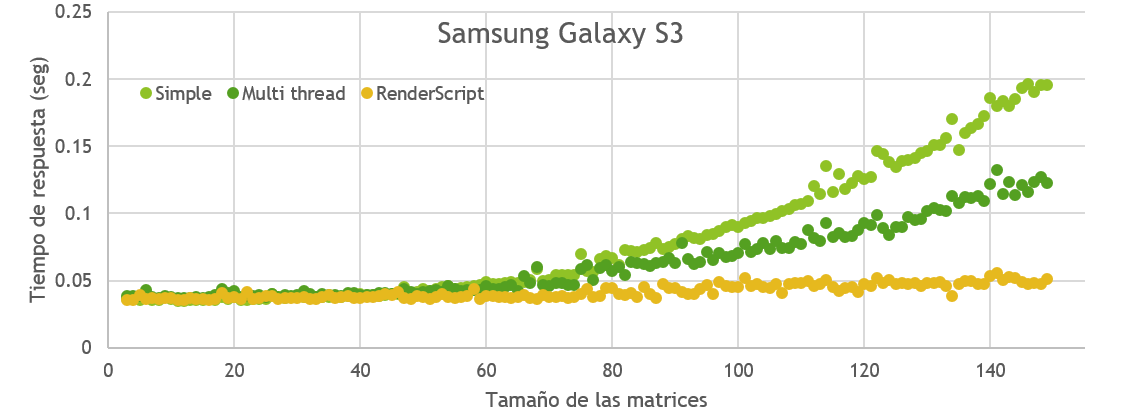
\includegraphics[scale=0.68]{images/Samsung}~
\par\end{centering}

\caption{Mediciones del tiempo de respuesta de los algoritmos de multiplicacion
de matrices\label{fig:Mediciones-del-tiempo-multiplicacion-de-matrices}}
\end{figure}


Respecto a los valores de tiempo registrados, puede notarse que el
tiempo de respuesta de los algoritmos crece polinomialmente respecto
al tamaño de las matrices, lo que coincide con la complejidad temporal
de la multiplicación de matrices que es $O(m\times n\times p)$. También
se observa que la versión del algoritmo multi-thread es mas eficiente
que la versión simple, y la versión usando el framework de RenderScript
es mucho más eficiente que las anteriores debido a la arquitectura
de los procesadores gráficos (GPU), que están diseñados para realizar
operaciones matriciales de coma flotante para el procesamiento de
gráficos y otros calculas.

Lo interesante de este escenario es que permite la creación de modelos
simples, por ejemplo, a partir de la técnica de regresión lineal,
ya que existe una correlación clara entre el tamaño de las instancias
del problema y el tiempo de ejecución que se puede aproximar con la
siguiente expresión:

\begin{center}
$tiempo_{C,D}=constante1+constante2\times m\times n\times p$
\par\end{center}

siendo $tiempo_{C,D}$ es el tiempo estimado de ejecución de un algoritmo
$C$ sobre un dispositivo $D$, para matrices de entrada $A_{m\times n}$
y $B_{n\times p}$.

En el cuadro \ref{tab:caso-de-estudio-1} se contrastan cada una de
las técnicas de regresión con cada uno de los componentes contemplados
en el caso de estudio:

\begin{table}[H]
\begin{doublespace}
\begin{centering}
\resizebox{1\textwidth}{!}{%
\begin{tabular*}{20cm}{@{\extracolsep{\fill}}|l|c|c|c|c|c|c|}
\hline 
 & \multicolumn{2}{c|}{{\large{}Algoritmo simple}} & \multicolumn{2}{c|}{{\large{}Algoritmo multi-thread}} & \multicolumn{2}{c|}{{\large{}Algoritmo RenderScript}}\tabularnewline
\hline 
 & {\large{}CC} & {\large{}RMSE} & {\large{}CC} & {\large{}RMSE} & {\large{}CC} & {\large{}RMSE}\tabularnewline
\hline 
{\large{}Linear Regression} & {\large{}0.9945} & {\large{}0.0042} & {\large{}0.9085} & {\large{}0.0156} & {\large{}0.5718} & {\large{}0.0002}\tabularnewline
\hline 
{\large{}MultiLayer Perceptron} & {\large{}0.9973} & {\large{}0.035} & {\large{}0.9187} & {\large{}0.0148} & {\large{}0.8578} & {\large{}0.013}\tabularnewline
\hline 
{\large{}SGD} & {\large{}0.9945} & {\large{}0.047} & {\large{}0.906} & {\large{}0.0209} & {\large{}0.5122} & {\large{}0.0061}\tabularnewline
\hline 
{\large{}Clusterer} & {\large{}0.996} & {\large{}0.012} & {\large{}0.9903} & {\large{}0.052} & {\large{}09929} & {\large{}0.0003}\tabularnewline
\hline 
\end{tabular*}}
\par\end{centering}
\end{doublespace}

\caption{Resultados obtenidos del primer caso de estudio. \label{tab:caso-de-estudio-1}}
\end{table}


En el cuadro \ref{tab:caso-de-estudio-1} se pueden apreciar las métricas
obtenidas a partir de los modelos calculados. A simple vista, se puede
apreciar que los modelos obtenidos para los dos primeros componentes
presentan una gran correlación, significando que el atributo buscado
(response time) tiene una gran dependencia de los atributos contemplados.
Esto concluye que el tamaño de las matrices multiplicadas influye
en el tiempo de respuesta para obtener el producto de dichas matrices.
En contraste, los modelos obtenidos para el algoritmo RenderScript
no presentan una correlación cercana a 1 como los demás algoritmos.
El componente RenderScript optimiza la ejecución de la multiplicación,
disminuyendo la relación entre el tamaño de la matriz y el tiempo
de respuesta.

En todos los escenarios presentados, se ha optado por el caso intermedio
de adaptación, considerando que el mejor modelo obtenido será aquel
que evite casos de overfitting o underfitting, focalizando el análisis
en los valores de \ac{CC} y \ac{RMSE} intermedios. Por lo tanto,
en este caso, el modelo más eficiente es el\emph{ Multilayer Perceptron.}



\begin{figure}[H]
\begin{centering}
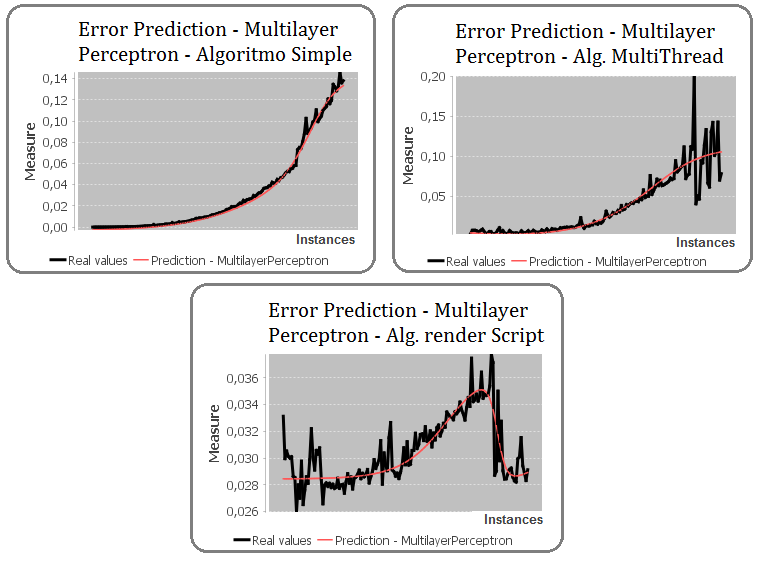
\includegraphics[scale=0.47]{images/response_neural_MM}
\par\end{centering}

\caption{Lineas de predicción en la herramienta Nekonata \label{fig:Lineas-de-predicci=0000F3n-matrix}}
\end{figure}



\section{Caso de estudio 2: algoritmos para el problema del viajante\label{subsec:Escenario-1:-Algoritmos}}

El problema del viajante o \ac{TSP} por sus siglas en inglés es un
problema clásico de optimización combinatoria que consiste en encontrar
la secuencia de caminos de menor distancia que debe recorrer un viajante
para visitar $n$ ciudades una y solo una vez cada una, empezando
por una ciudad cualquiera de ellas y regresando al mismo lugar del
que partió. En el campo de la teoría de complejidad computacional,
el problema del viajante, es un problema NP-Completo y es modelado
como un grafo de manera que las ciudades son sus vértices, los caminos
son las aristas y las distancias entre caminos son los pesos de las
aristas. Es un problema de minimización tras la búsqueda de un recorrido
completo que comienza y finaliza en un vértice específico y visita
el resto de los vértices exactamente una vez con coste mínimo. Existen
muchas variantes del problema, una de ellas se trata del \ac{TSP}
simétrico en el cual la distancia entre un par de ciudades es la misma
en cada dirección formando un grafo ponderado no dirigido. Esta variante
fue la versión considerada por la herramienta. 

Los componentes o algoritmos considerados para este dominio se describen
a continuación: 
\begin{description}
\item [{Best~Fit}] algoritmo heurístico que selecciona las ciudades de
acuerdo al costo de sus trayectos y son incorporadas al conjunto Solución
en base al cálculo de la distancia marginal de las intersecciones.. 
\item [{Nearest~neighbour}] partiendo de alguna ciudad arbitraria se analizan
todos los vértices adyacentes y aún no visitados, y se añade a la
solución aquel vértice cuya arista de costo sea la mínima. 
\item [{Lineal~Programming}] realiza una búsqueda exhaustiva simulando
el algoritmo backtracking, considerando restricciones y funciones
objetivo como fórmulas matemáticas. 
\item [{Prim}] crea un árbol de recubrimiento sobre el grafo y crea un
ciclo euleriano mínimo
\item [{Kruskal}] algoritmo similar a Prim en funcionamiento pero no en
ejecución, variando su complejidad.
\item [{Local~Transformations}] A través de un grafo hamiltoniano, se
analizan las aristas cruzadas obteniendo un nuevo ciclo.
\end{description}
Con el fin de garantizar instancias variadas del problema (diferentes
cantidades de ciudades, distintas representaciones y pesos) y para
la medición de los componentes, se utiliza la librería TSPLib\footnote{https://www.iwr.uni-heidelberg.de/groups/comopt/software/TSPLIB95/}
que contiene archivos con múltiples instancias del problema.. La librería
cuenta con 111 archivos de formato \emph{TSP}. Los ejemplos oscilan
desde 14 y hasta 18512 ciudades con un sólo ejemplo extremo de 85900,
y utilizan cuatro funciones de cálculo de la distancia entre ciudades:
distancia euclidiana, distancia geométrica, distancia pseudo euclidiana
y función techo. Para la obtención de las mediciones correspondientes,
se realizó una pre selección de 32 archivos que comprenden ejemplos
de entre 22 y 200 ciudades. Cabe destacar que fue necesaria la implementación
de un parser para el uso de los archivos. 

Por último, el dataset de mediciones obtenido para el entrenamiento
de modelos incluye atributos de las instancias del problema y propiedades
no-funcionales de la ejecución del componente. Los posibles atributos
de instancia son el número de ciudades, la cantidad de caminos y la
longitud de los mismo, sin embargo sólo se consideró la cantidad de
ciudades; y las propiedades de ejecución del componente son el tiempo
de respuesta, el valor solución, y la exactitud u optimalidad del
resultado, que es la razón entre el valor de la solución encontrada
y el valor óptimo de esa instancia del problema. 

Las pruebas fueron llevadas a cabo sobre los dispositivos móviles
Samsung Galaxy S4, S5 y S6. Los resultados presentados a continuación
consideran el desempeño de los aldoritmos sobre el dispositovo S4
a modo de referencia ya que los mismos no presentaban diferencias
significativas entre sí.

En la figura \ref{tab:response-caso-de-estudio-2-1} se puede observar
el tiempo de respuesta de los diferentes algoritmos considerando la
cantidad de ciudades. A simple vista se puede observar que los algoritmos
aproximados u óptimos tienen menor costo computacional debido que
no exploran la totalidad de ciudades para obtener la respuesta. Mientras
que los algoritmos exactos consumen más tiempo de respuesta ya que
hacen un análisis exhaustivo e incluso pueden requerir de algoritmos
auxiliares como el de ordenamiento. Gráficamente también se puede
observar un umbral en 50 ciudades, dividiendo los tiempos de respuesta
entre los cuales consideran la cantidad de ciudades como un factor
influyente y aquellos en los que pasa desapercibido.

\begin{figure}[H]
\begin{centering}
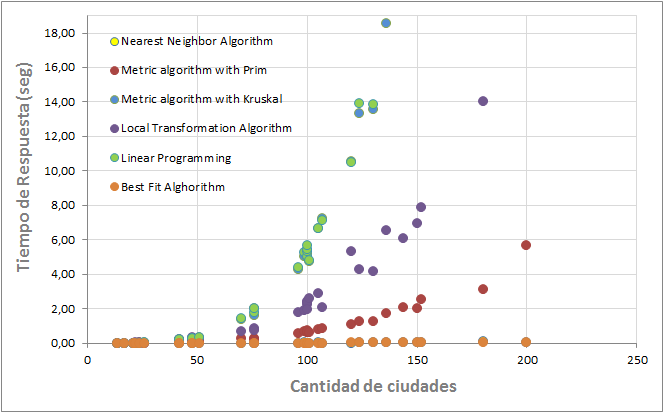
\includegraphics[scale=0.6]{images/S4}
\par\end{centering}

\caption{Mediciones de tiempo de respuesta de los algoritmos de resolución
del problema del viajante. \label{tab:response-caso-de-estudio-2-1}}
\end{figure}


A continuación se presentan los resultados de los modelos de regresión
del tiempo de respuesta:

\begin{table}[H]
\begin{doublespace}
\begin{centering}
\resizebox{1\textwidth}{!}{%
\begin{tabular*}{20cm}{@{\extracolsep{\fill}}|l|c|c|c|c|c|c|}
\hline 
 & \multicolumn{2}{c|}{{\large{}Best Fit}} & \multicolumn{2}{c|}{{\large{}Nearest Neighbour}} & \multicolumn{2}{c|}{{\large{}Linear Programming}}\tabularnewline
\hline 
 & {\large{}CC} & {\large{}RMSE} & {\large{}CC} & {\large{}RMSE} & {\large{}CC} & {\large{}RMSE}\tabularnewline
\hline 
{\large{}Linear Regression} & {\large{}0.98} & {\large{}0.0127} & {\large{}0.9281} & {\large{}0.0191} & {\large{}0.7535} & {\large{}17.8555}\tabularnewline
\hline 
{\large{}MultiLayer Perceptron} & {\large{}0.99} & {\large{}0.0034} & {\large{}0.9806} & {\large{}0.0050} & {\large{}0.9938} & {\large{}10.4876}\tabularnewline
\hline 
{\large{}\ac{SGD}} & {\large{}0.98} & {\large{}0.0045} & {\large{}0.9479} & {\large{}0.0090} & {\large{}0.8522} & {\large{}3.8502}\tabularnewline
\hline 
{\large{}Clusterer} & {\large{}0.98} & {\large{}0.0023} & {\large{}0.9920} & {\large{}0.0024} & {\large{}0.9961} & {\large{}1.5746}\tabularnewline
\hline 
{\large{}\ac{SMO}} & {\large{}0.99} & {\large{}0.0001} & {\large{}0.9999} & {\large{}0.0001} & {\large{}0.9999} & {\large{}0.1214}\tabularnewline
\hline 
\end{tabular*}}
\par\end{centering}
\end{doublespace}

\caption{Resultados obtenidos del caso de estudio dos \label{tab:caso-de-estudio-2}}
\end{table}


\begin{table}[H]
\begin{doublespace}
\begin{centering}
\resizebox{1\textwidth}{!}{%
\begin{tabular*}{20cm}{@{\extracolsep{\fill}}|l|c|c|c|c|c|c|}
\hline 
 & \multicolumn{2}{c|}{{\large{}Prim}} & \multicolumn{2}{c|}{{\large{}Kruskal}} & \multicolumn{2}{c|}{{\large{}Local Transformation}}\tabularnewline
\hline 
 & {\large{}CC} & {\large{}RMSE} & {\large{}CC} & {\large{}RMSE} & {\large{}CC} & {\large{}RMSE}\tabularnewline
\hline 
{\large{}Linear Regression} & {\large{}0.9835} & {\large{}1.1767} & {\large{}0.7553} & {\large{}17.0618} & {\large{}0.8835} & {\large{}4.4046}\tabularnewline
\hline 
{\large{}MultiLayer Perceptron} & {\large{}0.9923} & {\large{}0.1618} & {\large{}0.8993} & {\large{}8.8769} & {\large{}0.9950} & {\large{}0.7954}\tabularnewline
\hline 
{\large{}\ac{SGD}} & {\large{}0.9675} & {\large{}0.3545} & {\large{}0.9941} & {\large{}2.3924} & {\large{}0.9239} & {\large{}2.0863}\tabularnewline
\hline 
{\large{}Clusterer} & {\large{}0.9879} & {\large{}0.1823} & {\large{}0.9926} & {\large{}2.0626} & {\large{}0.9863} & {\large{}0.7248}\tabularnewline
\hline 
{\large{}\ac{SMO}} & {\large{}0.9999} & {\large{}0.0071} & {\large{}0.9999} & {\large{}0.0983} & {\large{}0.9999} & {\large{}0.0242}\tabularnewline
\hline 
\end{tabular*}}
\par\end{centering}
\end{doublespace}

\caption{Resultados obtenidos del caso de estudio dos \label{tab:caso-de-estudio-2-1}}
\end{table}


A partir de los cuadros \ref{tab:caso-de-estudio-2} y \ref{tab:caso-de-estudio-2-1}se
desprenden algunas conclusiones respecto al segundo caso de estudio.
En primer lugar, tanto el modelo de \emph{MultiLayer Perceptron} como
el de \ac{SMO} son, claramente, los mejores en cuanto a adaptación
al modelo. Ambos presentan una correlación de los datos cercano a
1 (\ac{CC}), lo que representa una buena precisión de los datos predichos
en relación a los reales. Como se ha se explicado en la sección\ref{sub:Ajuste-del-modelo:},
esto puede parecer lo más óptimo. Sin embargo, observando las métricas
y las curvas de errores, ambos modelos presentan el problema de overfitting. 

Teniendo esto en cuenta, se descartan las técnicas \emph{MultiLayer
Perceptron y }\ac{SMO} como mejores alternativas para este tipo de
problemas. A su vez, se descarta la técnica \emph{Linear Regression
}ya que presenta los niveles de correlación mas bajos y los errores
más altos.

La técnica que mejor se ajusta para este caso de estudio es el \ac{SGD}.\emph{
}A continuación, se presenta el comportamiento de este último con
respecto a los valores de referencia.

\begin{figure}[H]
\begin{centering}
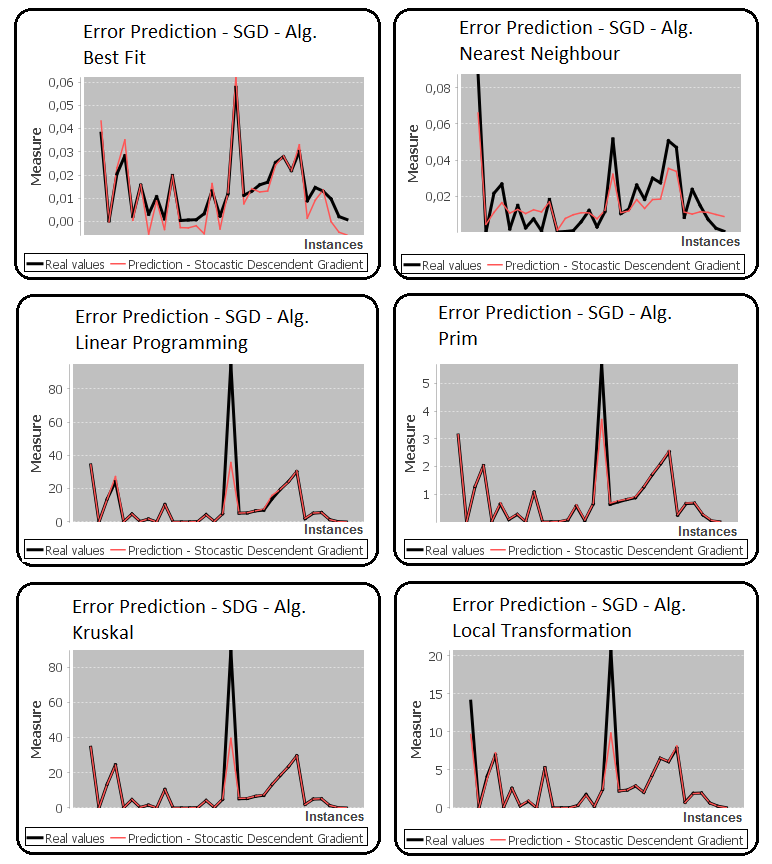
\includegraphics[scale=0.4]{images/response_SGD_TSPLIB}
\par\end{centering}

\caption{Lineas de predicción en la herramienta Nekonata}
\end{figure}



\section{Caso de estudio 3: servicios para detección de rostros\label{subsec:Escenario-2:-Servicios}}

El tercer escenario comprende un conjunto de servicios para la detección
de rostros en imágenes. La función que ofrecen es identificar las
regiones de una imagen que corresponden a rostros humanos. Hoy en
día muchas soluciones para detección de rostro se proporcionan como
servicios Web que, aunque no son tan eficientes y usables sin conexión
a Internet como las bibliotecas de software, resultan generalmente
más precisos y proporcionan características adicionales del rostro
como identificación de sonrisas, género e incluso estimaciones de
edad. Sin embargo, el rendimiento y la precisión de los servicios
varían según las propiedades de la imagen (tamaño, foco, oclusiones)
y contexto de ejecución (capacidad de procesamiento, conexión de red).
En la figura~\ref{fig:Ejemplo-de-detecci=0000F3n}~se muestra un
ejemplo de detección de rostros usando un servicio Web que incluye
identificación de sonrisas y estimación de edad para cada rostro.

\begin{figure}
\begin{centering}
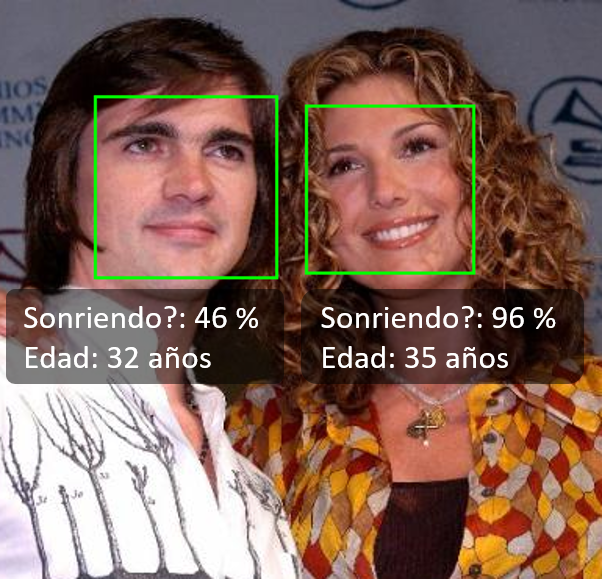
\includegraphics[scale=0.5]{images/ejemplo-de-deteccion-Microsoft-API}
\par\end{centering}

\caption{Ejemplo de detección de rostros en una imagen con el servicio de Microsoft
Face API.\label{fig:Ejemplo-de-detecci=0000F3n}}
\end{figure}


Los componentes considerados en el caso de estudio incluyen un servicio
local para dispositivos Android (Google Play Services face detector\footnote{https://developers.google.com/vision/})
y tres servicios Web (FaceRect API\footnote{http://apicloud.me/apis/facerect},
Sky Biometry API\footnote{https://skybiometry.com} y Microsoft Face
API\footnote{https://azure.microsoft.com/en-us/services/cognitive-services/}). 
\begin{description}
\item [{Google~face~API}] es una API para la detección de rostros en
imágenes y vídeos en tiempo real que forma parte del paquete de servicios
de Google Play para dispositivos Android. Estos servicios proporcionan
una gran variedad de APIs de Google, como geolocalización, servicios
de juegos y algoritmos de visión computacional como detección de rostros.
Al ejecutarse de manera local en el dispositivo, la funcionalidad
de detección de rostros no requiere conexión a Internet.
\item [{FaceRect~API}] es un servicio Web simple y gratuito para detección
de rostros en imágenes, consumido mediante interfaz \ac{REST}. 
\item [{Sky~Biometry~API}] es un servicio Web mas completo que incluye
características adicionales además de detección de rostros. También
es consumido mediante una interfaz \ac{REST}.
\item [{Microsoft~Face~API}] es un servicio Web en la nube que provee
algoritmos de detección y reconocimiento de rostros muy avanzados.
El servicio también se accede a través de una interfaz \ac{REST}.
El servicio forma parte de un grupo de APIs de inteligencia artificial
llamado Servicios Cognitivos.
\end{description}
Estos cuatro componentes fueron evaluados a partir de un subconjunto
de 290 imágenes pertenecientes al dataset llamado FDDB\citep{fddbTechReport}
con características muy variadas, incluyendo imágenes a color y escala
de grises, rostros de diferentes tamaños y posiciones, distintas resoluciones
de imágenes, etc. Como etapa de medición, cada servicio fue llamado
especificando una imagen y un conjunto de parámetros booleanos con
los que se le especifica al servicio que características se desean
extraer de los rostros (posición, sonrisa, edad, etc). Por cada invocación
se mide y registra el tiempo de respuesta en milisegundos. Las mediciones
del servicio Google face API fueron realizadas sobre un dispositivo
Lenovo K3 Note, mientras las mediciones de los servicios Web se realizaron
con la herramienta JMeter\footnote{http://jmeter.apache.org/}.

A diferencia de los casos de estudio anteriores, la correlación entre
el tiempo de respuesta y el tamaño de las instancias (medido, por
ejemplo, como la cantidad de pixeles de la imagen) es muy baja. Esto
se puede observar en la Figura~\ref{fig:Mediciones-del-tiempo-google-face-api},
donde se ilustran las mediciones del tiempo de respuesta para el servicio
de Google respecto al tamaño de las imágenes. Esta correlación es
aun peor es las mediciones de servicios Web, por lo que las propiedades
de las imágenes como su tamaño no fueron consideradas en el dataset
como variables para la predicción. Los atributos del dataset son conformados
por el valor de los parámetros booleanos con los que se invoca el
servicio, lo que conlleva a que existan muchas instancias conformadas
por atributos de igual valor que obtuvieron tiempos de respuestas
distintos.. En consecuencia, dos instancias análogas en sus requerimientos
podrían producir predicciones diferentes lo cual rompe el criterio
de unicidad de toda función matemática.

\begin{figure}
\begin{centering}
\includegraphics[scale=0.7]{\string"images/Google API\string".png}~
\par\end{centering}

\caption{Mediciones del tiempo de respuesta de Google Face API\label{fig:Mediciones-del-tiempo-google-face-api}}
\end{figure}


En el cuadro\ref{tab:caso-de-estudio-3}, se presentan los resultados
de correlación y error de los modelos de tiempo de respuesta obtenidos
para cada servicio:

\begin{table}[H]
\begin{doublespace}
\begin{centering}
\resizebox{1\textwidth}{!}{%
\begin{tabular*}{20cm}{@{\extracolsep{\fill}}|l|c|c|c|c|c|c|c|c|}
\hline 
 & \multicolumn{2}{c|}{{\large{}FaceRect API}} & \multicolumn{2}{c|}{{\large{}SkyBiometry API}} & \multicolumn{2}{c|}{{\large{}Microsoft Face API}} & \multicolumn{2}{c|}{{\large{}Google Face API}}\tabularnewline
\hline 
 & {\large{}CC} & {\large{}RMSE} & {\large{}CC} & {\large{}RMSE} & {\large{}CC} & {\large{}RMSE} & {\large{}CC} & {\large{}RMSE}\tabularnewline
\hline 
{\large{}Linear Regression} & {\large{}0.7000} & {\large{}153.6} & {\large{}0.08} & {\large{}637.54} & {\large{}0.41} & {\large{}71.78} & {\large{}0.6} & {\large{}59.17}\tabularnewline
\hline 
{\large{}MultiLayer Perceptron} & {\large{}0.7} & {\large{}153.52} & {\large{}0.09} & {\large{}637.83} & {\large{}0.58} & {\large{}64.04} & {\large{}0.66} & {\large{}55.54}\tabularnewline
\hline 
{\large{}\ac{SGD}} & {\large{}0.7} & {\large{}704.11} & {\large{}0.06} & {\large{}676.21} & {\large{}0.41} & {\large{}73.3} & {\large{}0.59} & {\large{}59.31}\tabularnewline
\hline 
{\large{}Clusterer} & {\large{}0.991} & {\large{}27.92} & {\large{} 0.13 } & {\large{}633.84} & {\large{} 0.56 } & {\large{}65.28} & {\large{} 0.78 } & {\large{}45.83}\tabularnewline
\hline 
\end{tabular*}}
\par\end{centering}
\end{doublespace}

\caption{Resultados obtenidos del caso de estudio tres. \label{tab:caso-de-estudio-3}}
\end{table}


Los datos exhibidos demuestran que el mejor modelo presentado para
predecir el tiempo de respuesta para el problema de detección de rostros
es el \emph{MultiLayer Perceptron}. El algoritmo no sólo ha arrojado
los valores más bajos del error de predicción sino que en todos los
casos, demuestra una buena adaptación a los dataset que por su naturaleza,
difieren en volumen de instancias, cantidad y tipo de atributos. 

A continuación, se presentan las lineas de predicción para demostrar
el desempeño de la técnica.

\begin{figure}[H]
\begin{raggedright}
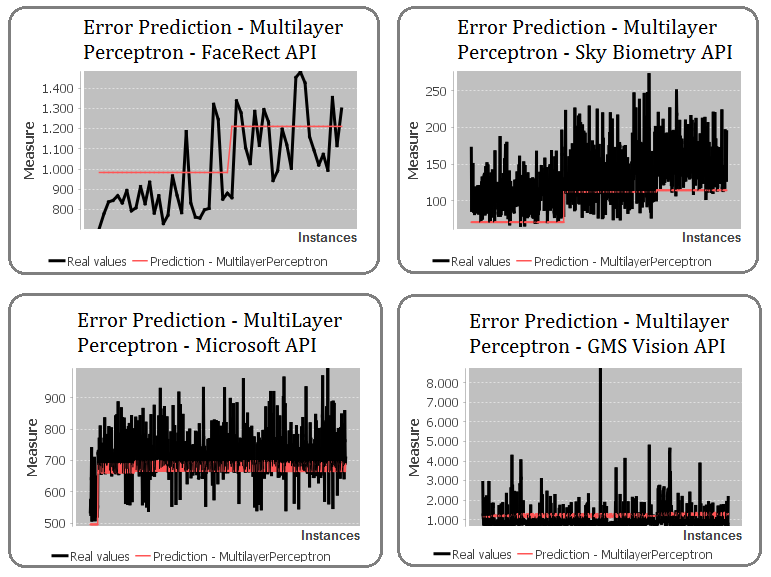
\includegraphics[scale=0.48]{images/response_face_lc}
\par\end{raggedright}

\caption{Lineas de predicción en la herramienta Nekonata \label{fig:Figura-comparativa-de-Multi}}
\end{figure}



\section{Análisis y discusión\label{sec:Analisis-y-discusi=0000F3n}}

En esta sección se analizan y discuten los resultados de las técnicas
entre sí. Es importante mencionar algunas consideraciones sobre la
técnica \ac{SMO} por las cuales se excluyó su aplicación sobre el
segundo y tercer caso de estudio. El desempeño de este algoritmo es
considerablemente superior en la calidad de sus respuestas, sin embargo
presenta algunas limitaciones para su uso; el desempeño del algoritmo
no es apto para formatos de dataset de cientos de instancias y múltiples
atributos, ya que en algunos casos la técnica requirió más de un día
de ejecución y en otros casos, sus resultados no pudieron ser visualizados.

En la evaluación del enfoque sobre los casos de estudio, solo se han
ejecutado los componentes sobre un número reducido de dispositivos.
Por lo tanto, no se consideraron características del dispositivo a
la hora de capturar mediciones y atributos para el entrenamiento de
modelos de predicción. Solo se consideraron atributos de los parámetros
de entrada de los componentes, además de su tiempo de respuesta, por
lo que los modelos solo generalizan la predicción sobre el dispositivo
en los que fueron tomadas las mediciones.

Considerando las mediciones tomadas en la primer etapa, se puede analizar
el comportamiento de los componentes respecto a un conjunto de entradas
particulares. Así, en el primer caso de estudio se puede observar
una gran dependencia entre el tamaño de la las instancias de la entrada
y el tiempo de respuesta. En el segundo caso, esta dependencia se
sigue observando pero mitigada mientras que en el último caso esta
dependencia es baja debido a la complejidad del problema de detección
de rostros. 

Si el desarrollador desea conocer el tiempo de respuesta aproximado
de un componente para un valor de entrada desconocido, utilizará el
modelo de predicción obtenido del aprendizaje. Así, en el primer y
último caso de estudio, el modelo de predicción más conveniente es
el MultiLayer Perceptron, mientras que en el segundo es el \ac{SGD}.
En cuanto a la correlación, se destaca que en el caso de estudio de
multiplicación de matrices, los algoritmos son sencillos y por lo
tanto poseen una correlación muy alta. Esto significa, que la técnica
determinó una buena relación entre las entradas de la función (entradas
del problema) y el atributo a predecir (tiempo de respuesta). En el
segundo caso, esta correlación es más baja debido a la mayor complejidad
del problema del viajante, y por último, en el caso 3, el problema
es más complejo no sólo por su objetivo sino porque no se han encontrado
atributos de las entradas que tengan buena correlacion con el tiempo
de respuesta. Esto significa una correlación mucho más baja y errores
más altos.



Cuanto mayor sea la correlación entre los datos de entrada del problema
y el tiempo de respuesta, menor es el grado de error en la predicción
ya que es más factible que el modelo encuentre una formula matemática
que describa la salida a partir de la entrada.


\section{Conclusiones \label{sec:Conclusiones}}

En este capítulo se presentaron distintos casos de estudio y se analizaron
los resultados producto de los mismos. En la primera sección se describió
el procedimiento llevado a cabo para la evaluación de la calidad de
los modelos predictivos construidos con técnicas de regresión. Luego,
se describieron los escenarios que conforman cada uno de los casos
de estudio donde se aplica el enfoque propuesto con las herramientas
implementadas. Finalmente, se analizan los resultados de los modelos,
de los que se extraen las siguientes consideraciones principales: 
\begin{itemize}
\item En caso de dataset formados por pocas instancias, como el caso de
estudio del problema del viajante, el comportamiento del \ac{SMO}
es similar al del Multilayer Perceptron. Sin embargo, es importante
destacar el efecto de overfit de ambos algoritmos, y particularmente
el tiempo de procesamiento que requiere el \ac{SMO}. 
\item En el caso de un dataset conformado por pocas instancias y buena correlación
entre el tiempo de respuesta y los datos de entrada, , como el caso
de estudio dos, la técnica \ac{SGD} presenta buenos resultados en
el modelo obtenido en relación al tiempo de ejecución que conlleva.
\item Analizando el desempeño de cada técnica y los resultados obtenidos,
se concluye que la mejor técnica para predecir el tiempo de respuesta
ha sido el Multilayer Perceptron. El mismo presenta buenos resultados
en datasets complejos y simples, generalizando el comportamiento de
los datos, como se puede apreciar en las figuras \ref{fig:Figura-comparativa-de-Multi}
y \ref{fig:Lineas-de-predicci=0000F3n-matrix}.\end{itemize}

